\documentclass[12pt,a4paper]{article}
\usepackage{graphicx}
\usepackage{wrapfig}
\usepackage{textcomp}

\title{Praktikum Physik - Hydrodynamik}
\author{Simon Marti, Patricia Schwab, Mirco Kocher}
\date{23.03.2012}

\newcommand{\subscript}[1]{$_{#1}$}
\newcommand{\B}[1]{B\subscript{#1}}
\newcommand{\V}[1]{V\subscript{#1}}

\parindent=0pt 
\begin{document}
\maketitle


\section*{Ziel}
\"Uberpr\"ufung der Druckabh\"angigkeit des Durchflusses f\"ur die Kapilaren verschiedener Druchmesser in Einzel-, Serie- und Parallel-Schaltung sowie bestimmung des Umschlagpunktes laminar-turbulent und der Rynoldszahl.

\section*{Motivation}
Der Versuch vertieft das Verst\"andnis f\"ur das Gesetz von Hagen-Poiseuille. Durch die Messung des Druchflusses f\"ur verschiedene H\"oheneinstellungen l\"asst sich zeigen, warum in kleinen Gef\"assen trotz ihrer gesamthaft gr\"osseren Querschnittsfl\"ache mehr Druch abf\"allt als in grossen Gef\"assen. Durch geringf\"ugige \"Anderungen k\"onnen Wirbel auftrete, welche Staupunkte verursachen und dadurch wiederum Anlagerungsprozesse beschleunigen. Die kleinsten Verschmutzungen oder Druck\"anderungen verursachen eine Abweichung von der optimalen Durchflussmenge. Verzweigungsstellen und Querschnitts-\"anderungen im Kapillarsystem sind besonders anf\"allig f\"ur ungewollte Analgerungen

\section*{Theorie}
TODO

\section*{Experiment I}

\subsection*{Aufbau und Ablauf}
\begin{center}
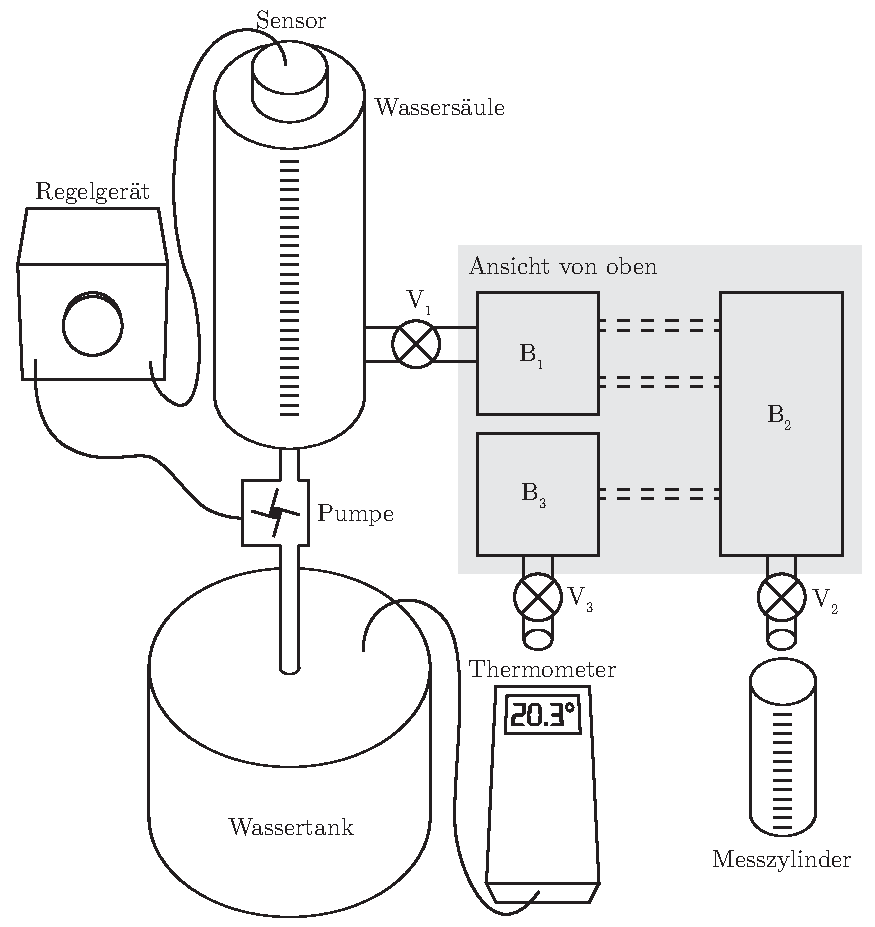
\includegraphics[width=11cm]{illustration.pdf}
\end{center}

Die aufgebaute Apparatur besteht aus wehreren Wasserbehältern die über R\"ohren und Schläuche miteinander verbunden sind. Zentral befinden sich drei Beh\"alter (\B{1}, \B{2} und \B{3}) die durch Kapillaren miteinander verbunden werden k\"onnen. An \B{2} und \B{3} befindet sich je ein Hahn durch welchen Wasser in einen Messzylinder geleitet werden kann (\V{2}, \V{3}). \B{1} ist mit einer Wassers\"aule verbunden die durch ein Regelgerät, welches mit einer Wasserpumpe und einem Wasserstand-Sensor verbunden ist, auf konstanter H\"ohe gehalten wird und oben offen ist. Das Wasser entnimmit die Pumpe aus einem offenen Beh\"alter in dem mithilfe eines elektronischen Thermometers die Wassertemperatur gemessen werden kann. Es befinden sich zusätzlich Entl\"uftungsventiele und Querverbindungen an den Beh\"altern die für die Versuche unwichtig sind und deshalb in der Grafik weggelassen wurden. Eine komplette \"Ubersicht der Ventiele findet sich im Script auf Abbildung 10.4.

Da die Vikosit\"at des Wassers von dessen Temperatur abh\"angt wird diese w\"ahrend der Durchf\"uhrung aller folgenden Augaben alle 15 Minuten gemessen.

\subsection*{Rohdaten}
\begin{tabular}{|l|l|}
\hline
$t$ [h]&$T$ [\textdegree C]\\
\hline
15:00&18.6\\
15:15&19.0\\
15:30&19.3\\
15:45&19.7\\
16:00&20.2\\
16:15&20.7\\
\hline
\end{tabular}


\section*{Experiment II}

\subsection*{Aufbau und Ablauf}
Zwischen \B{1} und \B{2} wird eine Kapillare mit $d$ = 1.01mm eingesetzt. Für mehrere H\"ohen $h$ der Wassers\"aule wird dann die Durchflussgeschwindigketi $Q$ gemessen indem f\"ur eine Minute das durchfliessende Wasser in einem Messzylinder gesammelt wird.

Bei diesem und allen folgenden Versuchen bedient Simon die Ventiele und die Stoppuhr und Mirco bestimmt jeweils die Wassermenge im Messzylinder.

\subsection*{Rohdaten}
\begin{tabular}{|l|l|}
\hline
$h$ [cm]&$Q$ [ml/min]\\
\hline
50&33\\
59.7&38.5\\
55&36\\
46.4&31\\
38.7&26\\
31.6&21\\
20.6&14\\
\hline
\end{tabular}

\subsection*{Auswertung}


\section*{Experiment III}

\subsection*{Aufbau und Ablauf}
Für eine gegebene H\"ohe der Wassers\"aule wird mit verschieden dicken Kapillaren zwischen \B{1} und \B{2} die Durchflussgeschwindigkeit $Q$ wie in Experiment II gemessen.

\subsection*{Rohdaten}
\begin{tabular}{|l|l|}
\hline
$d$ [mm]&$Q$ [ml/min]\\
\hline
1.01&33\\
0.61&5\\
0.84&17.25\\
1.23&65\\
\hline
\end{tabular}

\vspace{5pt}
$h$ = 50cm

\subsection*{Auswertung}


\section*{Experiment IV}

\subsection*{Aufbau und Ablauf}
F\"ur zwei Kapillare wird zuerst einzeln die Durchflussgeschwindigkeit $Q$ bestimmt, dann werden sie in Serie von \B2{1} zu \B{3} bzw. Parallel von \B{1} zu \B{2} eingesetzt und $Q$ wird erneut gemessen.

\subsection*{Rohdaten}

$d_1$ = 1.01mm

$d_2$ = 1.00mm

\vspace{5pt}
\begin{tabular}{|l|r|r|r|r|}
\hline
&K\subscript{1}&K\subscript{2}&Parallel&Seriell\\
\hline
$Q$ [ml/min]&33&33&68&17.25\\
$R$ []& & & & \\
\hline
\end{tabular}

\subsection*{Auswertung}


\section*{Experiment V}

\subsection*{Aufbau und Ablauf}
Eine Kapillare mit $d$ = 2.00mm wird zwischen \B{1} und \B{2} eingesetzt und f\"ur mehrere H\"ohen $h$ der Wassers\"aule wird die Durchflussgeschwindigkeit $Q$ bestimmt.

\subsection*{Rohdaten}
\begin{tabular}{|l|l|}
\hline
$h$ [cm]&$Q$ [ml/min]\\
\hline
59.7&274\\
42.8&242.5\\
28&190\\
11.8&97.5\\
35.2&220\\
50.5&256\\
20.4&150\\
15.4&120\\
25.5&178\\
30.8&202.5\\
\hline
\end{tabular}

\subsection*{Auswertung}


\section*{Diskussion}


\end{document}